\documentclass[11pt]{article}

% ------
% LAYOUT
% ------
\textwidth 165mm %
\textheight 230mm %
\oddsidemargin 0mm %
\evensidemargin 0mm %
\topmargin -15mm %
\parindent= 10mm

\usepackage[dvips]{graphicx}
\usepackage{multirow,multicol}
\usepackage[table]{xcolor}

\usepackage{amssymb}
\usepackage{amsfonts}
\usepackage{amsthm}
\usepackage{amsmath}

\usepackage{subfigure}
\usepackage{minted}
\usepackage{listings}

\lstset{
  breaklines=true,
}

\begin{document}
\noindent Homework Number: 02\\
Name: Yi Qiao\\
ECN Login: qiao22\\
Due Date: 1/24/2019\\
\section*{Answers}

\subsection*{encrypted text}
Since most characters is not printable, here is a screen shot with file opened with gedit.
\begin{figure}[h]
\centering
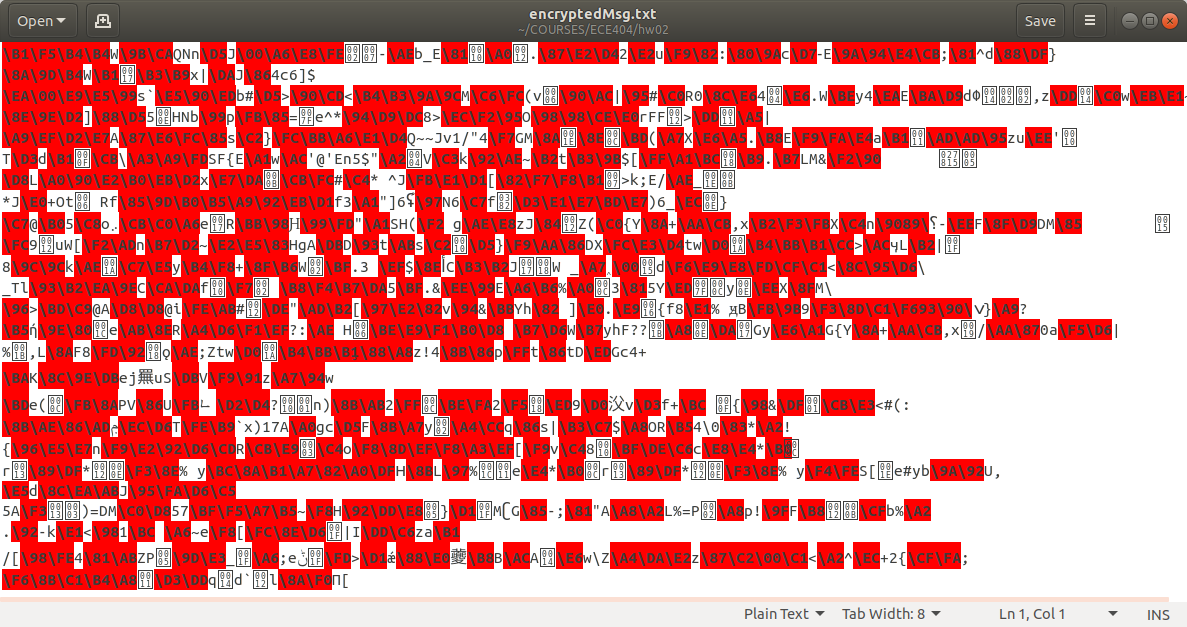
\includegraphics[width=0.8\linewidth]{encryptedMsg.png}
\end{figure}

\subsection*{encrypted ppm}
\begin{figure}[h]
\centering
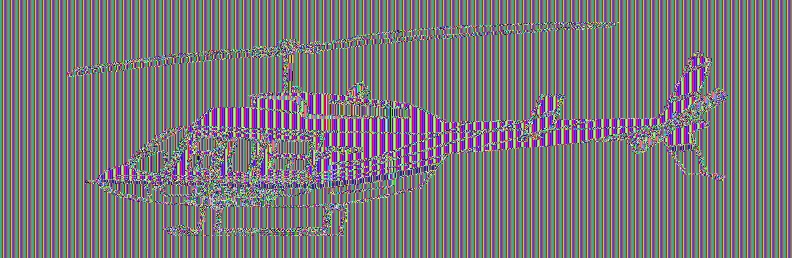
\includegraphics[width=0.8\linewidth]{image_enc.jpg}
\end{figure}
\pagebreak

\section*{Code}
\subsection*{DES\_text}
\inputminted[breaklines]{python}{DES_text.py}
\pagebreak
\subsection*{DES\_image}
\inputminted[breaklines]{python}{DES_image.py}

\end{document}